% ======================================
% TEORIA DE GRAFOS 
% ======================================
La teoría de grafos es una rama de las matemáticas y las ciencias de la computación orientada al estudio de las propiedades de los grafos, los cuales son abstracciones matemáticas utilizadas para modelar relaciones e interconexiones entre distintos objetos.

En definición un grafo en computación es una estructura de datos no lineal conformada por un conjunto de objetos llamados nodos los cuales están conectados por medio de aristas (o arcos). Utilizar grafos facilita la representación y el análisis de sistemas complejos dentro de los cuales se encuentran por ejemplo, las redes de transporte. 

\subsection{El problema del camino más corto}

Dentro de la teoría de grafos el Problema del Camino Más Corto o SPP por sus siglas en ingles (Shortest Path Problem), consiste en encontrar una ruta con el menor costo, distancia o tiempo entre dos vértices o nodos dentro de un grafo ponderado. El concepto de SPP es muy conocido dentro del panorama computacional ya que es comúnmente utilizado en diferentes aplicaciones o software de la vida cotidiana teniendo como mayor ejemplo al famoso Google Maps, siendo este el caso más conocido de la aplicación de la teoría de grafos en problemas SPP aplicando algoritmos de búsqueda para encontrar el camino más corto desde un nodo origen hacia un nodo destino por medio de una serie de aristas interconectadas entre múltiples nodos las cuales forman finalmente el grafo, dichos nodos representan las locaciones conocidas en el mundo real, las aristas los posibles caminos como calles o vialidades a disposición que interconectan los nodos y el grafo siendo la representación completa del mapa, zona, área o región mediante nodos y aristas. 

Dentro del ámbito de los grafos existen diversos tipos, y cada uno se adapta a diferentes necesidades o entornos por lo que es de vital importancia elegir de la mejor manera el tipo de grafo adecuado para el problema de esquematizar la zona de la alcaldía Gustavo A. Madero. Con el objetivo de solucionar la problemática planteada dentro del trabajo terminal, se evalúan los siguientes tipos principales de grafos:

\newpage

\subsection{Tipos de Grafos}

\subsubsection{Grafos dirigidos y no dirigidos} 
Dentro de un grafo dirigido las aristas tienen una dirección la cual indica el flujo de desplazamiento entre nodos, es decir, indican de que forma dentro del grafo podemos movernos entre nodos siguiendo la dirección de las aristas. Es común ver este tipo de grafo para flujo de trabajo o diagramas de procesos, donde el orden y la secuencia de los pasos importa. 

Con respecto a los grafos dirigidos, estos son su contraparte, por lo que las aristas no tienen dirección. Esto significa que la relación entre los nodos es bidireccional dando la posibilidad de poder transitar entre nodos en cualquier dirección por medio de las aristas. Este tipo de grafos suele utilizarse para representar relaciones reciprocas donde no importa la dirección o la secuencia entre nodos. 

\begin{figure}[h]
    \centering
    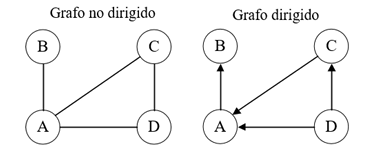
\includegraphics[width=0.6\textwidth]{figures/seccion3_3/grafo_dirigidoyno.png}
    \caption{Representación topológica de los grafos dirigidos y no dirigidos}
    \label{fig:grafo_dirigino-no}
\end{figure}

\subsubsection{Grafos ponderados y no ponderados} 
Existen grafos que incluyen pesos en sus aristas o valores numéricos los cuales representan el costo de la relación entre nodos. Usualmente este tipo de nodos son utilizados para representar relaciones donde el valor de las conexiones es importante para el problema, por ejemplo, en el caso de redes viales las aristas pueden integrar valores que representen la distancia entre nodos para después poder aplicar operaciones sobre dichos valores. 

En caso contrario el grafo no ponderado carece de información o etiquetas asociadas a las aristas. 

\begin{figure}[h]
    \centering
    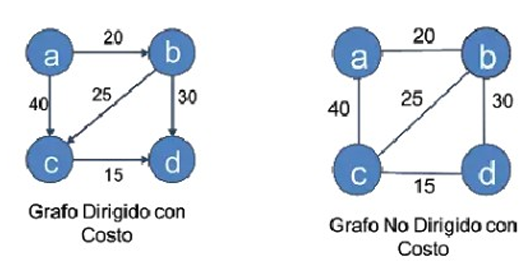
\includegraphics[width=0.8\textwidth, height=0.2\textheight, keepaspectratio]{figures/seccion3_3/grafo_ponderado_y_no_ponderado.png}
    \caption{Representación topológica de los grafos ponderados y no ponderados}
    \label{fig:grafon_pond_no}
\end{figure}

\subsubsection{Grafos cíclico y acíclicos}
Los grafos cíclicos contienen al menos un ciclo, un camino que comienza y termina en el mismo nodo. En los grafos cíclicos los vértices son componentes y las aristas representan conexiones lo que nos permite formar ciclos de corriente o un flujo de transición cíclico, es decir, que en alguno punto retorna al nodo de inicio donde se encontró por primera vez un ciclo. 

Al contrario los grafos acíclicos no tienen ningún ciclo. En la mayoría de los casos este tipo de grafos se utiliza para representar puramente relaciones y no secuencias. 

\begin{figure}[h]
    \centering
    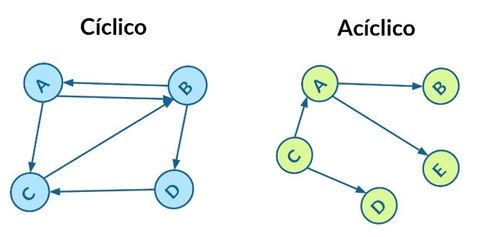
\includegraphics[width=0.8\textwidth, height=0.15\textheight, keepaspectratio]{figures/seccion3_3/grafio_ciclico_y_aciclico.png}
    \caption{Representación topológica de los grafos cíclicos y acíclicos}
    \label{fig:grafon_ciclico_no}
\end{figure}

\subsubsection{Grafos simples y multigrafos}
Un grafo simple se define como aquella estructura matemática donde un conjunto no vacío de vértices se interconecta a través de aristas únicas, restringiendo la existencia de trayectos paralelos entre un mismo par de nodos. 

Por su parte, un multigrafo representa una composición estructural de mayor complejidad, en la cual los nodos pueden interconectarse mediante múltiples aristas paralelas o alternativas. Esta característica permite modelar diferentes rutas o variables que coexisten entre los mismos puntos del entorno.

\begin{figure}[h]
    \centering
    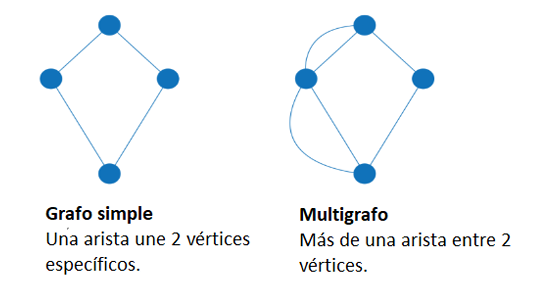
\includegraphics[width=0.8\textwidth, height=0.2\textheight, keepaspectratio]{figures/seccion3_3/grafo_simple.png}
    \caption{Representación topológica de los grafos simples y multigrafos}
    \label{fig:grafon_simp_no}
\end{figure}

\newpage

\subsubsection{Grafos conexos y no conexos}
En el análisis de redes topológicas, un grafo conexo se define como aquella estructura donde existe, al menos, un camino transitable entre cualquier par de vértices que lo componen. 

Por el contrario, un grafo no conexo presenta una fragmentación en su arquitectura, generando subgrafos o nodos aislados que carecen de enlaces con el entramado principal. 

\begin{figure}[h]
    \centering
    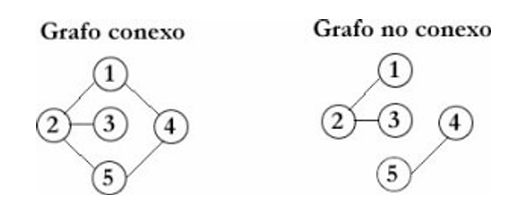
\includegraphics[width=0.8\textwidth, height=0.15\textheight, keepaspectratio]{figures/seccion3_3/grafo_conexo_y_no.png}
    \caption{Representación topológica de los grafos simples y multigrafos}
    \label{fig:grafon_con_no}
\end{figure}

\subsubsection{Elección y Justificación del tipo de grafo adecuado a la problemática presente}

Como se pudo apreciar hay bastantes tipos de grafos a tomar en cuenta sin embargo podemos decir con seguridad que lo más adecuado al problema es un grafo ponderado no dirigido con características del grafo simple, conexo y el cíclico. Al estar trabajando dentro de una demarcación territorial clasificada como localidad donde hay desplazamiento de vehículos e individuos constantemente, lo ideal es que los transcursos como calles o avenidas (aristas en el caso del grafo) estén sujetas a cierto peso debido a que esta información resulta útil para el calculo de rutas en la aplicación, en cuanto a la dirección realmente no es importante pues en la mayoría de transcursos el desplazamiento o traslado es bidireccional.

Cabe mencionar que en su mayoría la extensión territorial se rige por principios de un grafo simple ya que existe por lo menos un camino que conecte las múltiples ubicaciones o nodos del grafo. 

En cuanto al hecho de mantenerlo conexo es en relación a que en la localidad en la que el proyecto se esta desarrollando no se tienen zonas apartadas sin posible acceso, al contrario, todas las locaciones tiene un camino para trasladarse de un punto de origen a un punto de destino lo que evita caer en un grafo inconexo, ademas de que ser prácticamente imposible mapear un camino o ruta hacia nodos inaccesibles en caso de trabajar con zonas que se representen mediante grafos no conexos. También se integrarían elementos de un grafo cíclico ya que podemos retornar por múltiples caminos al nodo o locación de origen por ejemplo podemos volver a un punto de partida dando la vuelta a una manzana. 

\newpage

\subsection{Análisis de algoritmos de optimización en grafos}

\textbf{Algoritmos para problemas del camino más corto} \\
\label{AgSPP}

Existen una gran variedad de algoritmos que se encargan de resolver el \textbf{"Problema del camino más corto"} de múltiples formas, sin embargo, para este caso en particular no solo buscamos encontrar la ruta con menor costo de un punto a otro, también se integrara la inseguridad peatonal como variable compuesta de factores ambientales, sociales, estructurales y geográficos para obtener la generación de una ruta de transporte que tenga en cuenta los posibles factores de riesgo que pueden provocar un daño a la integridad de los peatones con la finalidad de balancear entre velocidad y seguridad para los usuarios. 

Es debido a la cantidad variada de algoritmos para problemas SPP (Shortest Path Problem) que debemos analizar los más adecuados al proyecto en busca de la mejor alternativa por lo que a continuación veremos en que consisten algunos de los algoritmos mas utilizados en la actualidad y con mayor eficiencia respecto a la optimización de grafos sin dejar de tomar en cuenta que tan benéficos y flexibles son para el proyecto considerando que deben trabajar con una variable extra, la inseguridad de los transcursos.

\subsubsection{Principales Algoritmos utilizados en problemas SPP}

En el ámbito de la informática y la computación existen múltiples algoritmos enfocados en la búsqueda de las rutas más optimas dentro de grafos ponderados sin embargo hay algoritmos que destacan sobre otros debido a su gran eficiencia y optimización provocando que en la actualidad sean un estándar al momento de resolver problemas de esta índole ya sea como base de un programa o como apoyo para desarrollar una mejora a partir de este grupo selecto de algoritmos, dentro los cuales se encuentran los siguientes: 

\subsubsection{Algoritmos de Origen Único (Single-Source)}
Dentro de esta sección se encuentran los algoritmos enfocados en buscar la ruta óptima desde un vértice inicial específico hacía uno o todos los demás nodos en la red. 

\begin{itemize}
    \item \textbf{Algoritmo de Dijkstra:} Garantiza encontrar la solución óptima global iterando siempre sobre el menor costo acumulado. Algunos algoritmos iteran sobre un grafo en busca de la solución más optima pero en veces no toman en cuenta todas las alternativas disponibles dentro del grafo y sus múltiples conexiones lo que provoca que al encontrar una solución al final de la iteración, esta misma sea un optimo local, es decir, una solución que es factible para esa ejecución en particular la cual tiene probabilidad de no ser la mejor de todas al no tomar en cuenta todas las alternativas. Dijkstra soluciona el problema del optimo local mediante el calculo de costo acumulado teniendo como único problema que el algoritmo no funciona para ponderaciones negativas lo que lo vuelve el estándar para redes viales urbanas donde las distancias físicas impiden la existencia de pesos negativos. 

    Dijkstra toma un nodo inicial (por ejemplo la dirección de un negocio o casa) y comienza a explorar todas las rutas posibles hacia el nodo de destino mientras lleva el calculo de la distancia acumulada en las diferentes posibilidades de trayectos los cuales se utilizaron para llegar al destino. Inicialmente parte del nodo de origen, "visita" primero al nodo más cercano y con menor coste para posteriormente trasladarse a dicho nodo y seguir repitiendo el proceso seleccionando siempre el camino de menor distancia acumulada conforme van aumentando los desplazamientos entre nodos. Es justo de esta forma como el algoritmo cada que llega a un nuevo "cruce", revisa, reconsidera y actualiza la distancia más corta registrada hasta el punto en el que se encuentra actualmente. En caso de encontrar una ruta más corta a una ubicación que ya había sido visitada por otro camino, el algoritmo reajusta el cálculo para reestructurar sus decisiones junto con la ruta que actualmente esta en ejecución hasta que finalmente consigue llegar al destino por medio del mejor camino posible \cite{dijkstra_udit}. 

    Dijkstra sigue siendo uno de los algoritmos de búsqueda para el camino más corto más importantes del panorama informático en general por lo que es una alternativa altamente útil al momento de aplicarlo sobre la propuesta de software "Prototipo de aplicación móvil para la generación de rutas peatonales seguras dentro de la alcaldía Gustavo A. Madero". 
    
    \item \textbf{A-Star (A*):} El algoritmo de A* se base en los principios fundamentales de Dijkstra que lo vuelven tan solido y añade una capa extra de inteligencia integrando la heurística o "intuición" como parte fundamental de la búsqueda \cite{dijkstra_udit}. 

    Antes de profundizar en el funcionamiento del algoritmo A*, primero debemos entender el concepto que se introduce con el uso de este algoritmo, la \textbf{heurística}. En el ámbito de la inteligencia artificial y la búsqueda en grafos, una heurística es un atajo mental, o mejor dicho, un conjunto de diferentes métodos, técnicas o estrategias que permiten solucionar un problema, tomar decisiones, emitir juicios o realizar descubrimientos de forma rápida y práctica.

    Las heurística nos permiten reducir drásticamente el tiempo y la energía invertida en la resolución de problemáticas sin embargo muchas veces resultan en conclusiones erróneas o imperfectas a causa de basarse en suposiciones, intuición o conocimientos parciales. Por lo tanto, pueden dar lugar a conclusiones sesgadas y juicios erróneos \cite{heuristica_que}.

    Para el caso especifico de A*, este combina dos variables al momento de estar explorando un grafo: por un lado la primera es la que propiamente Dijkstra introdujo, es decir, la distancia recorrida desde el inicio o "distancia acumulada" y, por otro lado, siendo la segunda variable la heurística que para este caso funge como la estimación de la distancia que falta hasta el destino. Por cada vez que A* realiza la búsqueda de su próximo movimiento, mantiene constantemente el calculo de la suma de lo que ya ha avanzado hasta el momento actual más lo que estima le queda por recorrer hasta llegar a la meta, hasta que finalmente llega al objetivo. Cabe mencionar que el uso de heurística ayuda al algoritmo a decidir de forma más rápida que camino es más conveniente de tomar para llegar a la meta pues "intuye" que su decisión podría ser optima a futuro sin dejar de lado el calculo real de distancia. 

    La heurística aplicada en A* y problemas de distancia como el de camino más corto en grafos, suele basarse en la distancia en linea recta hasta el destino u otro cálculo aproximado \cite{dijkstra_udit}. A* prioriza la exploración de los caminos que le parecen más prometedores para llegar al nodo de destino lo que causa la reducción de tiempo en el procesos de exploración visitando menos nodos que Dijkstra y por lo tanto logrando encontrar la solución en menor tiempo y mucho más rápido en muchos de los casos, a diferencia de la implementación normal de Dijkstra. Utilizar A* para el caso especifico del problema planteado en este trabajo terminal resulta extremadamente beneficioso debido a las condiciones que maneja y los requerimientos para su aplicación ya que otorga la posibilidad de plantear una heurística única que en conjunto con el calculo de distancias más la integración de variables de riesgo se pueda obtener una ruta en el menor tiempo posible lo más optimizada y segura para el usuario.  

    \item \textbf{Bellman-Ford:} A diferencia de Dijkstra, soporta aristas con pesos negativos y es capaz de detectar ciclos negativos infinitos. Su desventaja es una mayor complejidad computacional. Este algoritmo logra con éxito su cometido a través de la comprobación repetida de todas las aristas del grafo en busca de caminos más cortos, tantas veces como vértices haya en el grafo (menos 1) \cite{w3sch_bellmanford}. 

    Bellman-Ford también puede aplicarse a problemas de grafos donde no necesariamente hay aristas con pesos negativos, es decir, se puede utilizar en grafos con aristas que tengan exclusivamente pesos positivos al igual que con Dijkstra, sin embargo, para este tipo de casos es más recomendable utilizar Dijkstra ya que es más rápido y tiene menor complejidad. Pese a que el funcionamiento del algoritmo Bellman-Ford es relativamente sencillo no es recomendable aplicarlo en problemas de ruteo o vialidades donde los pesos negativos son inexistentes ya que es precisamente el funcionamiento de este algoritmo el que lo hace inviable para grafos con una gran cantidad de información como lo son mapas reales los cuales tienen un volumen de intersecciones (vértices |V|) y calles (|aristas |E|) de miles o decenas de miles. En esencia, el algoritmo comprueba todas las aristas a través de la matriz de adyacencia (estructura que representa las conexiones o aristas entre los vértices del grafo). En cada verificación, se busca determinar si es posible reducir la distancia hacia un nodo destino transitando a través del nodo origen y la arista que los conecta. Esta comprobación de todos los bordes se efectúa \textbf{V-1} veces, siendo \textbf{V} el número de vértices de las cual dispone el grafo utilizado. 

    Para el caso del presente trabajo terminal, las variables que conformarán el factor de "inseguridad" se modelaran como costos adicionales acumulativos en las aristas, dicho de otra manera, se desempeñaran como pesos positivos, nunca como bonificaciones que resten costo neto al trayecto. Dado que en este tipo de escenarios no existen aristas negativas, ciclos negativos o condiciones que modifiquen el peso de una arista hasta el punto de que su valor sea menor a cero, la principal ventaja teórica de Bellman-Ford queda sin utilidad, si entonces la principal ventaja de Bellman-Ford queda inútil, entonces no tendría caso tomarlo en cuenta dentro del problema ya que su implementación significa mayor tiempo de procesamiento reduciendo considerablemente la velocidad de la búsqueda gracias a la propia naturaleza en Bellman-Ford donde se examina todo el grafo y aristas repetidamente encontrando los caminos mínimos desde el origen hacia todos los demás vértices del grafo.

    \item \textbf{Greedy Best-First Search:} El algoritmo de búsqueda voraz primero el mejor o Greedy Best-First Search, es un método de búsqueda informada en inteligencia artificial esto quiere decir que trabaja mediante información adicional dentro de un entorno y sobre un problema para encontrar la solución más rápida. La búsqueda informada utiliza información heurística para guiar el proceso de búsqueda de manera más eficiente. 

    Greedy guía su búsqueda completamente en la heurística planteada en los grafos donde se aplica por lo que siempre encuentra un camino hacia un objetivo seleccionado eligiendo sin excepción a los nodos que parecen más prometedores en cada paso. Para el caso de búsqueda de rutas en mapas o zonas viales , este algoritmo resulta ineficiente ya que pese a su alta velocidad de ejecución peca de no siempre proporcionar la respuesta más optima debido a que se basa en un método de \textbf{selección voraz}, es decir, expande de inmediato el nodo que muestra el valor heurístico mas bajo, ignorando el costo real acumulado desde el inicio y pasando a explorar el nodo un valor heuristico más prometedor (muchas veces el de menor valor). 

    Como una de sus principales ventajas es que este algoritmo es rápido y eficiente en tiempo de cálculo lo que consume menor memoria que otros algoritmos más complejos sin embargo como ya se menciono, no siempre garantiza encontrar la ruta más corta u óptima y puede atascarse en óptimos locales si la heurística llegase a fallar. En este algoritmo, el costo de búsqueda es mínimo, pero aun así no lo convierte en una alternativa completa, puesto que puede conducir a un callejón sin salida. Se denomina "codicioso" porque en cada paso intenta acercarse lo máximo posible al objetivo \cite{greedy_voraz}.
    
    El hecho de que Greedy se base plenamente en suposiciones o heurística lo vuelve inestable para aplicaciones de mapas, que buscan obtener una ruta optima en todas las ejecuciones sin importar tanto la velocidad de ejecución por lo que es debido a lo anterior que la implementación de Greedy en el "Prototipo de aplicación móvil para la generación de rutas peatonales seguras dentro de la alcaldía Gustavo A. Madero" queda completamente descartado. 

    \item \textbf{Algoritmo de Rutas K de Yen:} El algoritmo de Yen entra dentro del tipo de algoritmos que están diseñados para encontrar el camino más corto en un grafo pero específicamente esta diseñado para encontrar \textbf{\textit{k}} caminos más cortos. En lugar de entregar unicamente la ruta matemáticamente perfecta, devuelve un ranking con las mejores alternativas (la opción 1, opción 2, opción 3... hasta llegar a \textbf{\textit{k}}). El algoritmo de Yen admite grafos ponderados con relaciones positivas y respeta las relaciones paralelas entre los mismos dos nodos al calcula múltiples rutas más cortas añadiendo el uso de la variable \textbf{\textit{k}}, donde \textbf{\textit{k}} es el número de rutas a calcular.  

    Funciona calculando primero la ruta principal utilizando Dijkstra o A*. Una vez que la tiene, comienza a bloquear artificialmente tramos o intersecciones de esa ruta principal para obligar al sistema a calcular desvíos. Después, evalúa todos estos desvíos, los ordena por su costo total, y extrae los siguientes mejores trayectos.

    La implementación del algoritmo de Yen tiene alta utilidad a nivel conceptual, pero presenta múltiples barreras y desafíos técnicos a tener en cuenta para la versión de nuestra aplicación móvil. Como principales ventajas tenemos que el uso del algoritmo de Yen puede dar la oportunidad de ofrecerle al peatón un listado de múltiples rutas con características que las diferencien entre si, delegando la decisión final al criterio del usuario y otorgando un atractivo a la experiencia de usuario al proporcionarle la opción de elegir entre diferentes alternativas de un trayecto. De igual forma si la ruta óptima llegase a presentar problemas u obstrucciones, el sistema ya tendría calculadas y listas las \textbf{\textit{k}} alternativas para re-dibujar el mapa al instante. 

    Lamentablemente el algoritmo de las K rutas sufre de algunas desventajas las cuales provocan problemas de rendimiento o eficiencia al momento de aplicarlos en situaciones de mapeo real incluyendo el caso particular de este trabajo terminal. Al momento de que Yen comienza a calcular las diferentes alternativas de rutas, regularmente estas opciones varían muy poco con respecto a la original ya que los cambios se provocan artificialmente dentro de la lógica lo que en términos reales podría representarse de la siguiente manera: En cuadriculas de calles, la segunda ruta más corta calculada por Yen suele ser idéntica a la primera en un 95 por ciento, desviándose solo por una calle paralela durante media cuadra. Esto computacionalmente es distinto, pero para el peatón no representa una alternativa real ni una mejora de seguridad.

    Otra gran desventaja es la alta exigencia de uso en el algoritmo de Yen pues ejecuta múltiples pasadas de búsqueda sobre el grafo. Si el polígono de evaluación es grande, el tiempo de respuesta pasaría de ser instantáneo a tardar varios segundos, arruinando la experiencia en tiempo real. En cuanto a las restricciones de uso del algoritmo, este no debe utilizarse cuando necesitemos considerar pesos negativos dentro de las estimaciones. Al igual que algoritmos similares de búsqueda de rutas optimas o cortas, no admite el hecho de que agregar relaciones pudiese hacer que una ruta sea más corta \cite{grapheverywhere_yen}.

    \textbf{El problema de recalculación continua}

    La problemática principal de implementar un algoritmo como el de K rutas de Yen es que no es tan flexible para trabajar en un entorno dinámico donde ciertas condiciones pueden afectar a la ponderación de aristas en el grafo. Para manejar eventualidades mientras el usuario ya está caminando, la industria no suele depender de rutas alternativas guardadas en memoria como lo hace el algoritmo de Yen, al contrario, la mejor práctica es configurar la lógica del software para escuchar activamente los cambios en el entorno; si por ejemplo en una calle dentro de la ruta trazada previamente, recibe una alerta mediante un sistema de \textbf{crowdmapping}, simplemente se lanza una nueva petición de A* desde la coordenada GPS actual del peatón. Al ser un algoritmo eficiente, la nueva ruta segura se dibuja en pantalla en milisegundos.  

    Lamentablemente el algoritmo de Yen realiza el calculo de rutas alternativas bajo la premisa de que el grafo se mantendrá en condiciones estáticas lo que lo vuelve muy ineficiente si hay que recalcular las rutas a mitad del viaje pues estaríamos forzando a la aplicación a realizar un re procesamiento de todas las rutas de Yen definidas ante una situación de emergencia como un reporte de crowdmapping, esto podría saturar los hilos de procesamiento de nuestra arquitectura. Yen también consume mucha memoria al bloquear nodos artificialmente y generar múltiples arboles de búsqueda significando un problema de rendimiento que aumentaría drásticamente si ahora lo integramos a un entorno dinámico donde un incidente puede llegar a cambiar las condiciones del grafo o inclusive también invalidar opciones de ruta previamente calculadas en una ejecución anterior de Yen. 

    En resumen se descarta la utilización del algoritmo de Yen debido a su tipo de funcionamiento para generar múltiples rutas precalculadas las cuales están diseñadas para mapas estáticos (como redes de fibra óptica), mientras mientras que la seguridad peatonal urbana requiere la flexibilidad de recálculo continuo que solo algoritmos como A* y Dijkstra pueden sostener eficientemente.

    % \item \textbf{Búsqueda en Anchura (BFS-Breadth-First Search:} La búsqueda en anchura o algoritmo BFS por sus siglas en ingles, es uno de los algoritmos más populares de recorrido de grafos en el campo de búsqueda no informada (también conocida como búsqueda a ciegas) donde se explora el espacio de búsqueda sin utilizar ninguna heurística ni conocimiento adicional sobre el objetivo. Se basa únicamente en la definición del problema y busca sistemáticamente una solución \cite{busqueda_info_no}.

    % BFS funciona realizando una exploración de todos los nodos en la profundidad que se encuentra en el momento de ejecución antes de pasar a los nodos del próximo nivel de profundidad, durante esta exploración en anchura se visitan primero los nodos vecinos, posteriormente los vecinos de estos, y así sucesivamente hasta llegar al ultimo nivel de profundidad donde ya se han explorado todos los nodos alcanzables. En términos generales el funcionamiento de BFS consiste en partir desde un nodo de origen seleccionado para después comenzar a visitar todos los nodos conectados directamente al nodo inicial, luego avanzar nivel por nivel hasta explorar todos los nodos posibles garantizando que cada nodo se visiten en orden de su distancia de origen \cite{bfs}. 

    % Como ya se menciono, BFS es un algoritmo que opera en el campo de la búsqueda no informada por lo que trabaja con grafos no ponderados y sin alguna heurística presente ya que no necesita de ninguna de estas variables para lograr su cometido el cual es explorar todo el grafo siguiendo cierto orden de exploración sin tomar en cuenta información adicional lo que lo vuelve eficiente para los casos específicos donde no es vital considerar información extra de un grafo pero se vuelve inútil su aplicación en entornos donde el grafo nos proporciona datos útiles para encontrar la ruta más corta de un punto a otro como lo es el caso de un mapa o una red de vialidad. 

    % La aplicación de BFS para el contexto en el que se desarrolla el prototipo de aplicación dentro de nuestro trabajo terminal resulta innecesaria que ya que este algoritmo ignoraría por completo variables como la distancia o inseguridad y optaría por escoger una ruta en base a la menor cantidad de aristas para llegar de un nodo a otro lo que vuelve inútiles nuestras variables principales las cuales son el cimiento principal para la construcción del prototipo de aplicación ya que se desea realizar la construcción de rutas en base a estas mismas, para cumplir con el objetivo principal de este trabajo el cual es generar rutas seguras y optimas para nuestros usuarios. 
    
    % \item \textbf{Búsqueda en Profundidad (DFS-Depth-First Search:} El funcionamiento del algoritmo DFS es similar al de BFS pues realmente el único cambio sustancial radica en el orden de exploración. La idea fundamental de DFS es que explora una rama del grafo o árbol lo más abajo posible antes de retroceder para explorar ramas alternativas \cite{dfs}. DFS explora primero todos los nodos en el nivel de profundidad que se encuentra hasta que no puede llegar más al fondo y empieza a explorar los nodos vecinos regresando a cada capa anterior de profundidad para explorar los caminos vecinos alternativos de la misma forma en la que inicialmente comenzó, es decir, continua explorando en profundidad hasta llegar a un camino sin alternativas y empezar a regresar a los niveles anteriores para seguir explorando en profundidad los nodos vecinos pendientes hasta recorrer el grafo por completo. 

    % DFS forma parte del campo de Búsquedas no informadas al igual que BFS por lo que también este algoritmo ignora por completo información adicional relacionada directamente con el grafo como lo son los pesos o heurísticas propuestas, recayendo en la misma conclusión que con BFS; su aplicación es innecesaria ya que no aprovecha los elementos cruciales del problema de grafos para representar un mapa donde el uso de ponderaciones y heurísticas es vital si queremos encontrar de forma optima una ruta de la manera más rápida y eficiente posible. 

    % Cabe mencionar que el hecho de que algoritmos como DFS y BFS pertenezcan a problemas de búsqueda de tipo no informada, provoca un cambio completamente de paradigma en cuento al tipo de soluciones que estaríamos obteniendo ya que ambos algoritmos garantizan encontrar una solución pero no aseguran que dicha opción sea la más optima o en su defecto la ruta más corta ya que no toman en consideración variables propias de grafos que entran en problemas de búsquedas informadas.  
    
    \item \textbf{Búsqueda en Anchura (BFS - \textit{Breadth-First Search}):} Es uno de los algoritmos más populares de recorrido de grafos en el campo de la búsqueda no informada (o búsqueda a ciegas). Funciona explorando sistemáticamente el espacio de búsqueda nivel por nivel; es decir, visita primero todos los nodos vecinos directos del origen antes de avanzar al siguiente nivel de profundidad, garantizando que cada nodo se visite en orden de lejanía \cite{busqueda_info_no, bfs}.
    
    Como ya se mencionó, al ser una búsqueda no informada, BFS trabaja con grafos no ponderados y no utiliza heurísticas. Aunque es eficiente en ciertos escenarios, su aplicación para el contexto de este Trabajo Terminal resulta innecesaria. Este algoritmo ignoraría por completo nuestras variables principales (como la distancia física y el índice de inseguridad) y optaría por escoger una ruta basándose únicamente en la menor cantidad de aristas. Esto descarta los cimientos del prototipo y nos impide cumplir con el objetivo principal del proyecto, el cual es generar rutas seguras y óptimas para los usuarios.
    
    \item \textbf{Búsqueda en Profundidad (DFS - \textit{Depth-First Search}):} El funcionamiento de DFS es similar al de BFS, pero el cambio sustancial radica en su orden de exploración. Su idea fundamental es explorar una rama del grafo lo más profundo posible hasta llegar a un camino sin alternativas, para luego retroceder y explorar las ramas vecinas pendientes hasta recorrer el grafo por completo \cite{dfs}.
    
    Al igual que BFS, DFS forma parte de las búsquedas no informadas, recayendo en la misma conclusión: su aplicación es inviable para este modelo porque ignora la información adicional del grafo. 
    
    Cabe mencionar que el hecho de que algoritmos como DFS y BFS pertenezcan a este paradigma provoca un cambio total en el tipo de soluciones obtenidas. Aunque ambos algoritmos garantizan encontrar una solución (un camino hacia el destino), no aseguran que dicha opción sea la más óptima ni la más corta, ya que desperdician por completo las ponderaciones del mapa y las heurísticas que son vitales para encontrar un trayecto de forma eficiente.

\end{itemize}

\subsubsection{Algoritmos para todos los pares (APSP All-Pairs Shortest Path ):}

Existe un categoría de algoritmos de ruta más corta poco conocida que pese a su poca fama resulta bastante importante en el tema de los algoritmos en grafos ya que introduce un nuevo enfoque para atacar el problema del camino más corto. Estamos hablando de los algoritmos de la familia All-Pairs Shortest Path (APSP) enfocándose ahora en calcular en simultaneo todas las rutas optimas disponibles entre todas las combinaciones posibles de nodos dentro de un grafo. A diferencia de los algoritmos de origen único donde se busca hallar una ruta especifica de un punto A hacia un punto B, en los algoritmos para todos los pares se calcula una matriz completa con toda la información acerca de las rutas más cortas entre todos los pares de nodos, es decir, dentro de la matriz cualquier nodo ya tiene su distancia minina resulta hacia cualquier otro punto del grafo. 

Pese a la utilidad que proporciona este nuevo enfoque algorítmico para resolver el problema del camino más corto, su aplicación dentro del presente trabajo puede llegar a perjudicar gravemente la eficiencia de la aplicación ya que presenta problemas técnicos que pueden conflictuar con el prototipo de aplicación, llegando a afectar negativamente el rendimiento del proyecto. Estas desventajas se analizaran de la mano de la explicación de los dos algoritmos para todos los pares que se detallarán a continuación:

\begin{itemize}

    \item \textbf{Floyd-Warshall:} Pertenece a la categoría de algoritmos de caminos más cortos para todos los pares (APSP, por sus siglas en inglés). Utiliza un enfoque de programación dinámica para construir una matriz bidimensional, actualizando iterativamente las distancias al evaluar cada vértice como un nodo intermedio, hasta encontrar las rutas óptimas entre todas las combinaciones posibles en la red \cite{gfg_floyd_warshall, gfg_floyd_warshall_cpp, gfg_floyd_warshall_c}. Posee una complejidad computacional de $O(V^3)$, siendo adecuado principalmente para grafos densos.
    
    Sin embargo, su integración en este Trabajo Terminal resulta inviable. Modelar la red vial de la alcaldía Gustavo A. Madero implica trabajar con un grafo de gran extensión, lo que provocaría un consumo excesivo de memoria para almacenar la matriz de distancias. El factor más crítico radica en la variable de "inseguridad": al ser dinámica y alimentada mediante \textit{crowdmapping}, cualquier actualización en los pesos de las aristas obligaría al sistema a recalcular la matriz entera desde cero, lo que colapsaría el rendimiento del prototipo.

    \item \textbf{Algoritmo de Johnson:} Es una alternativa de tipo APSP diseñada para ser asintóticamente más rápida que Floyd-Warshall en grafos dispersos, logrando una complejidad de $O(V^2 \log V + VE)$ \cite{enjoyalgorithms_graphs}. Su funcionamiento es híbrido: primero utiliza el algoritmo de Bellman-Ford sobre un nodo temporal para eliminar aristas de peso negativo mediante una técnica de reponderación, y posteriormente ejecuta el algoritmo de Dijkstra desde cada nodo para calcular la matriz de distancias finales \cite{book_algoritmos_johnson}.
    
    A pesar de su mayor eficiencia estructural frente a Floyd-Warshall, su aplicación se descarta para este proyecto por dos motivos fundamentales. En primer lugar, el grafo del entorno de estudio no contempla ponderaciones viales negativas, volviendo inútil la fase de reponderación de Bellman-Ford. En segundo lugar, al seguir siendo un algoritmo APSP, calcular exhaustivamente todos los pares en una red dinámica sujeta a constantes cambios por reportes de seguridad provocaría tiempos de ejecución inaceptables. Para el cálculo de rutas punto a punto con pesos dinámicos, los enfoques APSP son ineficientes.

    % \item \textbf{Floyd-Warshall:} El algoritmo de Floyd pertenece a la categoría de los algoritmos para caminos más costos para todos los pares (APSP). El funcionamiento del este algoritmo consisten en ir manteniendo una matriz bidimensional que representa las distancias entre nodos. Inicialmente, esta matriz se llena utilizando únicamente las aristas directas entre nodos. Posteriormente, el algoritmo actualiza gradualmente estas distancias comprobando si existen rutas más cortas a través de nodos intermedios \cite{gfg_floyd_warshall}. 

    % Utiliza un enfoque de programación dinámica para comparar todas las rutas posibles a través del grafo. La matriz que utiliza registra las rutas más cortas entre todos los pares de vértices y sirve para representar dichas distancias entre cada par de vértices, estableciendo inicialmente la distancia a infinito para todos los pares excepto para la diagonal (distancia de un vértice a sí mismo), que se establece en cero \cite{gfg_floyd_warshall_cpp}. 
    
    % El algoritmo a su vez se encarga actualizar iterativamente esta matriz considerando cada vértice como un punto intermedio y comprobando si existe una ruta más corta entre un origen y un destino que pase por dicho vértice, repitiendo este procesa hasta agotar todas las combinaciones posibles de vértices en la red \cite{gfg_floyd_warshall_c}. 

    % Floyd-Warshall se desenvuelve correctamente para la mayoría de los tipos de grafos, a excepción de los que tienen ciclos negativos, por lo que su uso es flexible en este ámbito. Cabe mencionar que, sin importar el número de aristas de un grafo, este algoritmo maneja una complejidad computacional de $O(V^3)$, donde $V$ es el número de vértices, lo que da como resultado que sea más adecuado para grafos donde el número de aristas se aproxima al número máximo posible de conexiones que pueden existir entre sus nodos; a estos grafos se les conoce como grafos densos.

    % Lamentablemente ahora es cuando entramos a los conflictos que puede implicar integrar algoritmos del tipo APSP para nuestro problema del camino más corto considerando pesos y la variables de "inseguridad" la cual provoca cambios constantes dentro de las ponderaciones del grafo. Integrar el algoritmo de Floyd-Warshall al proyecto implicar tener en cuanta que la alta complejidad temporal que maneja este algoritmo lo vuelve lento para grafos muy grandes por lo que es posible tengo problemas de rendimiento en grafos relacionados con representaciones viales de extensiones territoriales relativamente grandes como lo pueden ser las secciones GAM de la Gustavo A. Madero. Cabe mencionar que requiere mucha memoria para mantener la matriz de distancias considerando que aquí se integra toda la información de las rutas entre todos y cada uno de los pares de nodos, problema que puede escalar aun más al trabajar en un grafo extenso como lo es el caso de este trabajo terminal. Este ultimo punto es tal vez la problematica más importante ya que al integrar una variable como lo es la "inseguridad" dentro del grafo, estamos obligando a los algoritmo a re calcular rutas en caso de sufrir modificaciones en las aristas conforme estén activos los reportes de crowdmapping lo que obligaría al sistema a re calcula toda la matriz desde cero suponiendo que se implemente Floyd-Warshall como algoritmo principal, es por esto que su uso queda descartado dentro del proyecto. 

    % \item \textbf{Algoritmo de Johnson:} El algoritmo de Johnson también se aplica en problemas donde el objetivo es encontrar los caminos más cortos entre todos los pares de vértices en un grafo. Se desempeña eficientemente dentro de grafos con pesos no negativos y resulta una alternativa eficiente al algoritmo de Floyd-Wharshall cuando el grafo es disperso, es decir, grafos en donde el numero de aristas es relativamente menor en relación al número de vértices. Cuando hablamos de dispersión de un grafo estamos hablando de su densidad de aristas la cual se define como la relación entre el número de aristas del grafo y el número máximo de aristas posibles. En un grafo disperso, la densidad de aristas es relativamente baja \cite{enjoyalgorithms_graphs}.

    % El algoritmo de Johnson calcula los caminos más costos entre todos los pares en tiempo $O{(V^2lgV + VE)}$. En comparación al algoritmo de Floyd-Warshall o el método de elevación de matrices al cuadrado, el algoritmo de Johnson es asintóticamente más rápido que los dos métodos anteriores dentro de grafos dispersos. Este algoritmo utiliza como subrutinas tanto el algoritmo de Dijkstra como el algoritmo de Bellman-Ford para devolver una matriz con todos los pesos de los caminos más cortos para cada par de vértices o bien informa si el grafo tiene un ciclo de peso negativo. Johnson logra su cometido a través de la técnica de reponderación de aristas o resignación de pesos, la cual funciona de la siguiente manera: Si todos los pesos $w$ de las aristas de un grafo $G=(V, E)$ donde de $V$ es el número de vértices y $E$ es el número de aristas del grafo, son no negativos, es posible implementar el uso de Dijkstra para encontrar los caminos más cortos entre todos los pares de vértices una vez desde cada vértice; utilizando una cola de prioridad mínima del montículo de Fibonacci, el tiempo de ejecución de todos los pares se mantiene igual en $O{(V^2lgV + VE)}$ \cite{book_algoritmos_johnson}.

    % En general el funcionamiento del algoritmo de Johnson se podría describir de la siguiente manera: primero crea un nodo temporal que se conecta absolutamente a todos los cruces topológicos (nodos) del mapa (grafo) con un costo de 0, después entra en acción el algoritmo de Bellman-Ford para ejecutarse desde el nodo temporal con el propósito de ajustar los pesos de todo el grafo para eliminar cualquier arista con peso negativo sin alterar las proporciones de las rutas más cortas. Una ves que el grafo ya fue procesado al completo por Bellman-Ford y todos los pesos de las aristas son positivos, Johnson ejecuta el algoritmo de Dijkstra desde cada uno de los nodos del mapa para que finalmente se restauren los pesos matemáticos a sus valores originales y se entregue una matriz completa de $V x V$ con todas las distancias resultas.

    % Pese a las ventajas que puede llegar a proporcionar el uso del algoritmo de Johnson con respecto a Floyd-Warshall, en el contexto especifico de un entorno dinámico donde el grafo esta constantemente sujeto a cambios dentro de las ponderaciones provoca altos problemas de rendimiento ya que sigue manteniendo el principio de calcular una matriz con todos los caminos cortos del grafo, lo que se traduce en menor velocidad de ejecución al estar re calculando la matriz cada que se presente una cambio en las ponderaciones de nuestro grafo en relación con la variable de "inseguridad". Cabe mencionar que en nuestro modelo no manejamos pesos negativos por lo tanto el atractivo de re-ponderación de Bellman-Ford que ofrece Johnson se vuelve inútil para nuestro caso de estudio en el trabajo terminal. El simple hecho de que el algoritmo de Johnson forme parte de los algoritmos APSP (All Pairs Shortest Path) lo vuelve inviable en proyectos similares al presente en este documento, lo que descarta su implementación dentro de la aplicación. 
    
\end{itemize}

\subsubsection{Búsqueda Bidireccional; un nuevo enfoque en problemas de la búsqueda del camino más corto:}

Los algoritmos de búsqueda clásicos operan construyendo un árbol de búsqueda sobre un grafo, comenzando la exploración desde un nodo inicial hasta alcanzar un nodo destino a través de una ruta óptima. En contraste, la \textbf{Búsqueda Bidireccional} consiste en la ejecución de dos exploraciones simultáneas: una hacia adelante desde el nodo origen y otra hacia atrás desde el nodo destino, con el objetivo de encontrar el camino interconectado más rápido en tiempo de ejecución.

Suponiendo que se busca trazar una ruta desde un nodo $A$ hacia un nodo $B$, el enfoque bidireccional despliega los algoritmos de búsqueda de manera concurrente en ambos extremos. La ruta final se establece al detectar el cruce entre ambas exploraciones; es decir, en el momento exacto en que las fronteras de expansión de los dos árboles de búsqueda (tanto de $A$ como de $B$) se intersectan en un nodo intermedio.

Este enfoque proporciona la ventaja de encontrar en la mayoría de los casos, la ruta óptimas más rápido que los algoritmos de origen único, sin embargo, requiere un diseño cuidadoso, especialmente en lo que respecta los criterios de parada lo que lo vuelve más difícil de implementar y depurar \cite{baeldung_bidirectional_search}. 
    
El principal impedimento radica en el manejo de nuestra variable dinámica de "inseguridad". En algoritmos heurísticos bidireccionales (como el $A^*$ Bidireccional), diseñar una función heurística admisible y consistente para ambos extremos es matemáticamente complejo. Además, la condición de parada se vuelve un problema crítico: el hecho de que las fronteras de búsqueda del origen y el destino se crucen en un nodo intermedio no garantiza que esa sea la ruta más segura u óptima cuando los pesos de las aristas cambian constantemente por los reportes de \textit{crowdmapping}.

Resolver estas colisiones y garantizar la ruta óptima con pesos dinámicos añadiría una sobrecarga computacional innecesaria al servidor. El sistema responde de mejor manera al procesamiento de redes viales utilizando búsqueda unidireccional informada para este caso en particular por lo que queda descartado el uso de búsqueda bidireccional.

\subsubsection{Selección del Algoritmo de Ruteo}

Tras analizar los principales algoritmos de ruteo para solucionar el problema del camino más corto, se ha optado por implementar \textbf{A*} en conjunto con \textbf{Dijkstra} dentro del desarrollo del prototipo de aplicación ya que ambos demostraron ser los más adecuados para el proyecto con base en la teoría vista en \ref{AgSPP}.

